% document formatting
\documentclass[10pt]{article}
\usepackage[utf8]{inputenc}
\usepackage[left=1in,right=1in,top=1in,bottom=1in]{geometry}
\usepackage[T1]{fontenc}
\usepackage{xcolor}

% math symbols, etc.
\usepackage{amsmath, amsfonts, amssymb, amsthm}

% lists
\usepackage{enumerate}

% images
\usepackage{graphicx} % for images
\usepackage{tikz}

% code blocks
\usepackage{minted, listings} 

% verbatim greek
\usepackage{alphabeta}

\newcommand{\dd}{\text{d}}
\newcommand{\pr}{\text{Pr}}

\graphicspath{{./assets/images/Week 10}}

\title{02-712 Week 10 \\ \large{Biological Modeling and Simulation}}
 
\author{Aidan Jan}

\date{\today}

\begin{document}
\maketitle

\subsection*{Ergolic Graphs}
An Ergolic graph is one where every state is reachable from every other state with a non-zero probability.  Suppose we have an ergodic graph with states:
\[Q = (q_1, q_2, q_3, q_4, q_5)\]
which includes transitions in both directions between:
$(q_1, q_2), (q_2, q_3), (q_3, q_4), (q_4, q_5), (q_2, q_5)$.  Note that $q_2$ has the highest degree in the graph (degree 3).
\begin{center}
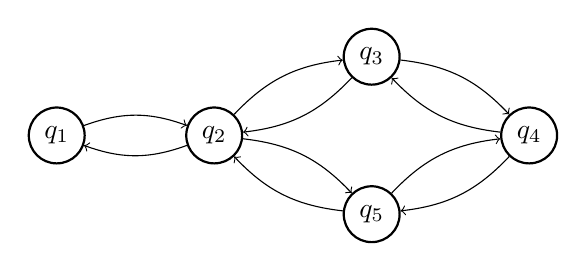
\begin{tikzpicture}
    \node[thick, circle, draw] at (0, 0) (q1) {$q_1$};
    \node[thick, circle, draw] at (2, 0) (q2) {$q_2$};
    \node[thick, circle, draw] at (4, 1) (q3) {$q_3$};
    \node[thick, circle, draw] at (6, 0) (q4) {$q_4$};
    \node[thick, circle, draw] at (4, -1) (q5) {$q_5$};
    
    \draw[->, bend left=20] (q1) to (q2); \draw[->, bend left=20] (q2) to (q1);
    \draw[->, bend left=20] (q2) to (q3); \draw[->, bend left=20] (q3) to (q2);
    \draw[->, bend left=20] (q3) to (q4); \draw[->, bend left=20] (q4) to (q3);
    \draw[->, bend left=20] (q4) to (q5); \draw[->, bend left=20] (q5) to (q4);
    \draw[->, bend left=20] (q5) to (q2); \draw[->, bend left=20] (q2) to (q5);
\end{tikzpicture}
\end{center}
We will use a model called the metropolis model on this graph:
\begin{enumerate}
	\item Given a state $q_i$, pick a neighbor $q_j$ uniformly at random with probability $\frac{1}{d}$ (or $q_i$ again with probability $1 - \frac{d_i}{d}$ if $d_i < d$)
	\item If $E_j < E_i$, move to $q_i$.
	\item If $E_j > E_i$, move with probability $e^{-(E_j - E_i) / kT}$
	\item Go to step 1.
\end{enumerate}
Remember that $E$ represents the "energy" of a state.\\
What the description above means is that, let a probability be on every edge.  All transitions add up to less than or equal to 1.  If less than 1, then the probability of a self loop is the remaining fraction.

\subsubsection*{Detailed Balance}
Detailed balance means that $\pi_i p_{ij} = \pi_j p_{ji}$.  Essentially, the probability of being in $i$ and moving to $j$ is equal to the probability of being in $j$ and moving to $i$.  This property is present in \textit{every} metropolis model.\\\\
This reason for this is that every metropolis model satisfies the \underline{Kolmogarov Criterion}.  Basically, imagine a set of nodes in a cycle.  If moving from one node to another, where there is a \textit{decrease} in energy, then we would move with a probability of $\frac{1}{d}$.  If there was an \textit{increase} of energy, then we would move with a probability of $\frac{1}{d} e^{-\Delta_i / kT}$.\\\\
The total probability of going around the entire cycle would be
\[\left(\frac{1}{d}\right)^{k + 1} e^{-\frac{1}{kT} \sum \Delta_i},\quad \text{ where $i$ represents entries where energy increases}\]
Now, if we go around the cycle the other way, then all the signs flip.  The number of $\frac{1}{d}$ factors stay the same, but the deltas in the exponential term will be all those that did not appear originally.  However, since a manhattan model has the property that the probability of $\pi_i p_{ij} = \pi_j p_{ji}$ as described earlier, these two exponentials must be equal.  Therefore, every manhattan model must exhibit detailed balance.

\section*{Weighted Sequence Sampling}
Suppose we have a DNA sequence, and we want to calculate dinucleotide frequency bias.  For example, consider the target sequence $GG$, and we have the following sequences:
\begin{itemize}
	\item $ACAGTAC$ - 1
 	\item $ACGGTAC$ - 2
	\item $ACGGTGG$ - 4
	\item $ACGGGAC$ - 4
\end{itemize}
A weight is the number of $GG$'s present in the target sequence, assuming 

We can model this with a metropolis model.  
\begin{itemize}
	\item Let the state set $Q = \{A, C, G, T\}^n$.
	\item Transitions: $NN \cdots (n) \cdots NN \rightarrow NN \cdots (N') \cdots NN$
	\item Given $q_i$:
	\begin{enumerate}
	    \item Pick base $j$ uniformly from $1$ to $n$.
	    \item Pick new nucleotide uniformly at random with probability $\frac{1}{3}$
	    \item Compare number of $GG$.  If we have $\dots GAG \dots \rightarrow \dots GGG \dots$, then $\Delta GG = 2$.  (Moving backwards would be $-2$)
	    \item If $\Delta_{GG} > 0$, accept the change.
	    \item If $\Delta_{GG} < 0$, accept with probability $2^{\Delta_{GG}}$
    \end{enumerate}
\end{itemize}

\subsection*{Metropolis for Optimization}
Suppose we have an objective function $I(c)$.  We can calculate a score $e^{-I(c) / z}$ for every state, and use a Metropolis model to pick the highest probability state out of the entire model by tracking the amount of time spent on each state.

\subsection*{Gibbs Sampling}
\[p(x_1, x_2, \dots, x_n) = \pr\{X_1 = x_1, X_2 = x_2, \dots, X_n = x_n\}, \quad X_1 \in R_1\]
[FILL]

Algorithm:
\begin{enumerate}
	\item Pick $x_j$ uniformly at random from $1 \dots n$.
	\item Sample $x_j$ from the conditional density $\pr \{x_j' | x_1, \dots, x_{j}, x_{j + 1}, \dots, x_{n}\}$
	\item Repeat (go to step 1)
\end{enumerate}

\subsubsection*{Example: Ising Model}
Suppose we have a row of magnets that are close to each other.  Each magnet either points up or down.  Same repels, opposites attract.  \\\\
Let the magnets be $X_1, \dots, X_n$, where $X_i \in \{+1, -1\}$.  To use the Gibbs sampling model,
\begin{enumerate}
	\item Pick $i \leftarrow \lceil u[0, n]\rceil$
	\item Sample of $X_i$
	\[\pr\{X_i = -1 | X_j \neq X_i\} = \left(e^{((-1) x_{i - 1} + (-1) x_{i + 1}) g/kT}\right) / \left(e^{((-1) X_{i - 1} + (-1) X_{i + 1}) g/kT} \cdot e^{(X_{i - 1} + X_{i + 1}) g/kT}\right)\]
    \[\pr\{X_i = +1 | X_j \neq X_i\} = \left(e^{(x_{i - 1} + x_{i + 1}) g/kT}\right) / \left(e^{((-1) X_{i - 1} + (-1) X_{i + 1}) g/kT} \cdot e^{(X_{i - 1} + X_{i + 1}) g/kT}\right)\]
    \item (note that the denominators of both are the same)
\end{enumerate}

\subsection*{Importance Sampling}
Given $Q = \{q_1, \dots, q_n\}$ and $\Pi = \{\pi_1, \dots, \pi_n\}$
\begin{enumerate}
	\item Make $\hat{\Pi} = \{\hat{\pi_1}, \dots, \hat{\pi_n}\} = \hat{\Pi_i} = \frac{\pi_i w_i}{\sum \pi_i w_i}$
	\item Sample from $\hat{\Pi}$
	\item Scale estimates $\hat{\pi_1}, \dots, \hat{\pi_n}$ by $w_i$
	\item ($w_i$ represents weights.)
\end{enumerate}

\subsection*{Umbrella Sampling}


\end{document}